% Lista02.tex
% !TeX root = L02_RelFinal.tex
\section*{Lista de Exercícios 2}
\addcontentsline{toc}{chapter}{Lista de Exercícios 2}

\noindent \textbf{Data:} 04/09/2026

\begin{enumerate}
    \item Considere uma placa delgada com dimensões $L$ (em $x$), $H$ (em $y$) de um material qualquer que possui propriedades constantes: $k_{x}$, $k_{y}$, $\rho$, $c$ (sendo $k_{x}$ e $k_{y}$ da mesma ordem, mas possuem valores diferentes). A placa está a uma dada condição inicial de temperatura $T=T_{amb}$ bem como os seus contornos são mantidos a $T=T_{amb}$. Em $t=0$ uma geração de calor em unidade de $(W/m^{3})$ passa a ocorrer na posição central da placa $\left(\frac{L}{2}; \frac{H}{2}\right)$ (considere como um ponto).
    \begin{enumerate}
        \item Esboce a geometria deste problema;
        \item Apresente o modelo para este problema (hipóteses simplificativas, condições de contorno e equação governante);
        \item Proponha uma malha espacial para este problema;
        \item Aplique o MVF para o volume de controle central (ao redor de $\left(\frac{L}{2}; \frac{H}{2}\right)$) e apresente a equação discretizada na sua forma geral.
    \end{enumerate}

        \item Na equação da conservação da quantidade de movimento de Brinkman-Frochheimer, apresentada abaixo na sua forma unidimensional ao longo de um eixo longitudinal, proponha uma linearização para o termo fonte.
        \begin{equation*}
            \frac{\rho}{\varepsilon}\left(\frac{\partial u}{\partial t}\right) = -\frac{\partial P}{\partial x} - \frac{\mu}{K}\,u - \frac{c_{E}\,\rho}{K^{0.5}}\,u|\,u|
        \end{equation*}
        em que $\rho$ é a densidade, $\mu$ a viscosidade, $\epsilon$ a porosidade, $\frac{\partial P}{\partial x}$ o gradiente de pressão, $K$ a permeabilidade do meio poroso, $c_{E}$ a constante de Ergun do meio poroso, e $u$ a velocidade.
        
        Considere que $\frac{\partial P}{\partial x}$ é uma função do tempo, dada por $\frac{\partial P}{\partial x} = f(t)$. Logo, o termo da pressão não precisa de discretização espacial.

    \item Considere o problema ilustrado na figura abaixo. Nele, temos uma barra de metal com comprimento de 0,2 m e área de seção transversal de 0,1 $m^{2}$ com as propriedades descritas na imagem. Na posição $x=0$ a barra é submetida a um fluxo constante de $100~W/m^{2}$ ao passo que na posição $x=L$ a temperatura é prescrita e igual a 300 K. Não há geração.
    
    \begin{center}
        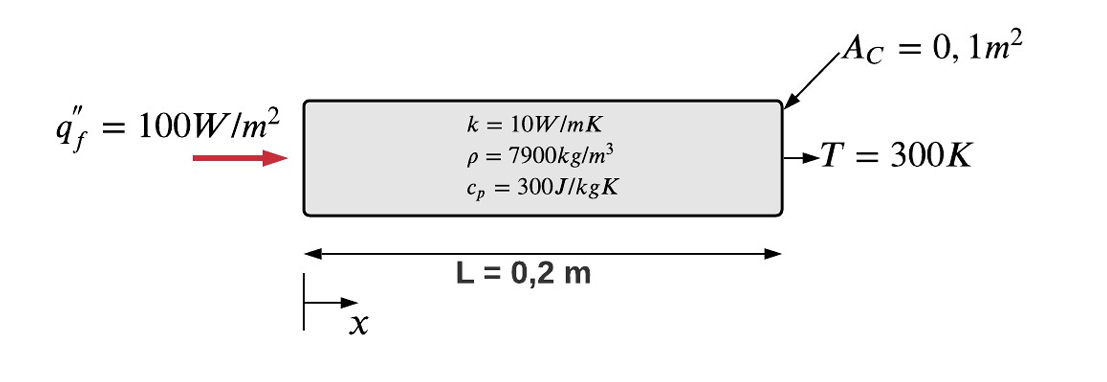
\includegraphics[width=0.8\textwidth]{Q3.png}
    \end{center}
    \FloatBarrier

    Resolva o problema de condução transiente 1D até encontrar a condição de regime permanente. Utilize:
    \begin{itemize}
        \item A formulação explícita;
        \item Implemente as condições de contorno utilizando o balanço nos volumes de fronteira;
        \item Resolva no MS-Excel, de preferência.
    \end{itemize}
    Para a análise:
    \begin{itemize}
        \item Resolva o problema utilizando 5 volumes, 10 volumes e 20 volumes;
        \item Para cada malha, encontre o máximo valor de incremento no tempo que garanta o critério de von Neumann (OBS: esse valor será encontrado para um dos volumes de fronteira, assim, deve-se avaliar os volumes internos e os de fronteira);
        \item Obtenha a solução convergida para cada malha em estudo, utilize como critério de convergência para cada volume, em que $k$ é o tempo atual e $k-1$ o tempo anterior:
        \begin{equation*}
            |T^{k}-T^{k-1}| < 0,001
        \end{equation*}
        \item Encontre o tempo total necessário para convergir para cada uma das malhas;
        \item Compare o resultado convergido com a solução em regime permanente;
        \item Disserte sobre o que pode ter ocorrido no resultado quando se compara as 3 malhas propostas.
        \item Na sequência, utilize como critério de convergência:
        \begin{equation*}
            |T^{k}-T^{k-1}| < 0,00001
        \end{equation*}
        \item Disserte sobre o novo resultado e sobre a importância de avaliar o critério de convergência. Englobe na sua ponderação o tempo final encontrado para obter o resultado convergido.
    \end{itemize}

    \item Resolva numericamente a equação abaixo, usando uma formulação explícita. Use uma malha com 5 pontos (dois sobre as fronteiras) e admita as temperaturas iguais a 1 nas fronteiras esquerda e direita. A condição inicial é $T(x)=0$ em todo o domínio. Considerando $\alpha = 1$ e $\Delta x = 1$, use $\Delta t$ igual a 0,25; 0,50 e 0,75, avance a solução para 6 intervalos de tempo para cada caso. Comente os resultados.
    \begin{equation*}
        \frac{\partial T}{\partial t} = \alpha\frac{\partial^{2}T}{\partial x^{2}}
    \end{equation*}

    \item Considere uma placa delgada com dimensões $L$ (em $x$), $H$ (em $y$) de um material qualquer que possui propriedades constantes: $k$, $\rho$, $c_{p}$. A placa está a uma dada condição inicial de temperatura $T=T_{amb}$, e os seus contornos são mantidos sob as condições apresentadas na figura abaixo. Desconsidere geração de calor. UTILIZANDO A FORMULAÇÃO TOTALMENTE IMPLÍCITA:
    \begin{enumerate}
        \item Apresente o modelo para este problema (hipóteses simplificativas, condições de contorno e equação governante);
        \item Aplique o MVF em todos os volumes. Para os volumes nos contornos aplique o método do balanço de energia apresentado na aula.
    \end{enumerate}
    \textit{Note que: neste problema serão necessários discretizar nove equações diferentes para cada volume finito ilustrado na figura: 1 para os volumes internos e 8 para as condições de contorno.}

    \begin{center}
        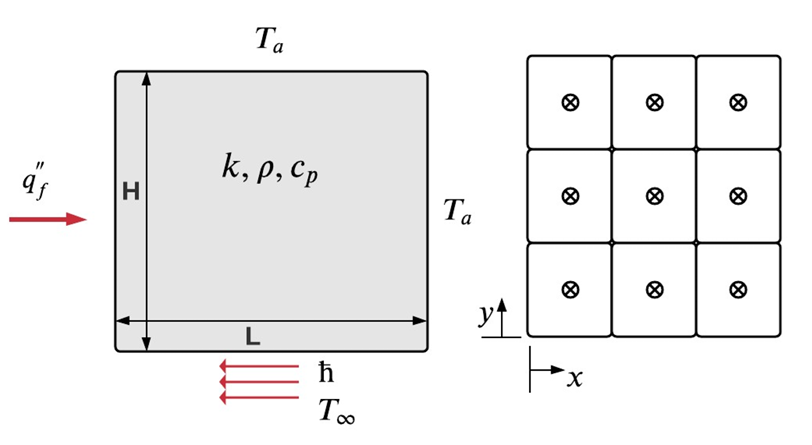
\includegraphics[width=0.8\textwidth]{Q5.png}
    \end{center}
    \FloatBarrier

\end{enumerate}

\section*{Resolução}
\subsection*{Questão 1}
\subsubsection*{a) Esboce a geometria do problema.}
A Figura~\ref{fig:esb1} mostra um esquemático da placa do problema de condução de calor da Questão 1. Na ilustração, a geração de calor está localizada no ponto \textit{P}.

\vspace{0.5cm}

\begin{center}
    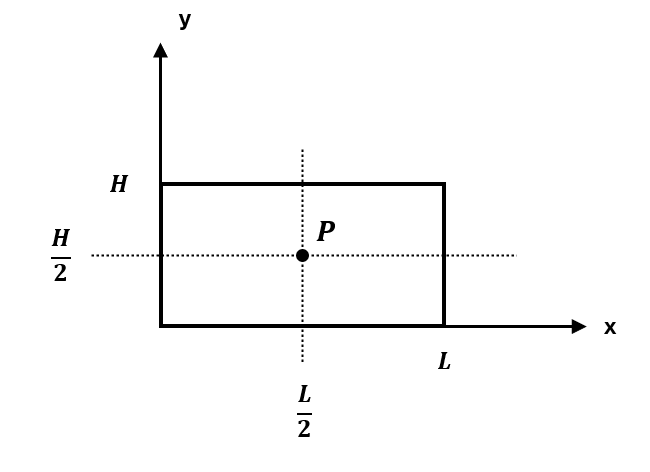
\includegraphics[width=0.5\textwidth]{esb1.png}
    \captionof{figure}{Geometria para condução de calor bidimensional com fonte geradora}
    \label{fig:esb1}
\end{center}
\FloatBarrier

\subsubsection{b) Apresente o modelo para este problema (hipóteses simplificativas, condições de contorno e equação governante).}
As hipóteses simplificativas que permitem a resolução do problema pelo método de volumes finitos são:
\begin{itemize}
    \item Propriedades constantes e uniformes: $k_{x}$, $k_{y}$, $\rho$ e $c$.
    \item Meio sólido, homogêneo, contínuo e em repouso, sem advecção, sem mudança de fase e sem deformação.
    \item Placa delgada e de espessura uniforme sem troca de calor na direção z $\left(\dfrac{\partial T}{\partial z} = 0\right)$.
    \item A geração, informada por unidade de volume, é admitida como atuante em uma região de dimensões pequenas frente a $L$ e $H$, representada na malha pelo volume de controle central. Dessa forma, a potência total gerada é, portanto, $S_{C}\,\Delta x\,\Delta y$.
\end{itemize}

\textbf{Condições de contorno:}

$T(0,y,t) = T(L,y,t) = T(x,0,t) = T(x,H,t) = T_{amb}$

\textbf{Condição inicial:}

$T(x,y,0) = T_{amb}$

\textbf{Equação governante:}

$\rho\,c\,\dfrac{\partial T}{\partial t} = k_{x}\,\dfrac{{\partial}^{2} T}{\partial x^{2}} + k_{y}\,\dfrac{{\partial}^{2} T}{\partial y^{2}} + S_{C}(x,y)$

\subsubsection{c) Proponha uma malha espacial para este problema.}
Propõe-se uma malha cartesiana estruturada com arranjo \textit{cell center}, em que os nós ocupam os centros dos volumes de controle e as faces dos volumes extremos coincidem com os contornos da placa. Adota-se número ímpar de volumes em ambas as direções, de modo que a posição $(L/2\,;H/2)$ coincida com o centro de um volume, e não com uma face ou um vértice.

Essa exigência decorre da forma como o termo fonte entra no balanço, por meio da integral $\int_{V}{S_{C}}\,dV$, que representa a potência gerada no interior do volume: caso a geração estivesse sobre uma face, ela pertenceria simultaneamente a dois volumes e sua repartição dependeria de convenção arbitrária. Propõe-se, ainda, refinamento nos volumes vizinhos ao central, região em que os gradientes de temperatura são mais intensos.

\subsubsection{d) Aplique o MVF para o volume de controle central (ao redor de $\left(\dfrac{L}{2};\dfrac{H}{2}\right)$) e apresente a equação discretizada em sua forma geral.}
Forma geral:


$A_{P}\,T_{P} = \left(A_{E}\,T_{E}^0 + A_{W}\,T_{W}^0 + A_{N}\,T_{N}^0 + A_{S}\,T_{S}^0 + \left[A_{P}^0 - A_{E} - A_{W} - A_{N} - A_{S}\right]\,T_{P}^0\right)\,\Delta t + S_{C}\,\Delta x\,\Delta y$


\subsection*{Questão 2}

Como a equação apresentada não possui derivadas espaciais da velocidade, não há fluxos a serem avaliados nas faces do volume de controle. Assim, todo o lado direito da equação constitui o termo fonte:

\begin{center}
    $S = -\dfrac{\partial P}{\partial x} - \dfrac{\mu}{K}\,u - \dfrac{c_{E}\,\rho}{K^{0,5}}\,u\,|u|$
\end{center}

A linearização consiste em escrever esse termo como uma função linear da incógnita do volume de controle:

\begin{center}
    $S = S_{C} + S_{P}\,u_{P}$
\end{center}

em que $S_{C}$ é a parcela tratada de forma explícita e $S_{P}$ é o coeficiente que multiplica a incógnita, sendo transferido para o coeficiente central da equação discretizada. Os dois coeficientes são obtidos avaliando-se o termo fonte e a sua derivada em um valor estimado da velocidade, $u_{P}^{*}$, tomado do passo de tempo anterior:

\begin{center}
    $S_{P} = \left(\dfrac{dS}{du}\right)^{*} \qquad ; \qquad S_{C} = S\left(u_{P}^{*}\right) - \left(\dfrac{dS}{du}\right)^{*}u_{P}^{*}$
\end{center}

Exige-se ainda que $S_{P} \le 0$. Como esse coeficiente é transferido para o lado esquerdo da equação, resultando em $A_{P} = A_{P}^{0} - S_{P}$, um valor negativo aumenta o coeficiente central e favorece a estabilidade, enquanto um valor positivo o reduz, podendo anulá-lo ou torná-lo negativo.

Analisando os três termos separadamente:

\vspace{0.5cm}
\begin{itemize}
    \item [1 - ]O termo de pressão é função apenas do tempo e não depende da velocidade, portanto sua derivada em relação a $u$ é nula e ele é incorporado integralmente à parcela constante:
    \begin{center}
        $S_{C} = -f(t) \qquad ; \qquad S_{P} = 0$
    \end{center}
    \vspace{0.5cm}
    \item [2 - ]O segundo termo já é linear em $u$, de modo que sua linearização é exata. Sua derivada é constante e negativa, pois $\mu$ e $K$ são positivos, atendendo à condição de sinal:
    \begin{center}
        $S_{C} = 0 \qquad ; \qquad S_{P} = -\dfrac{\mu}{K}$
    \end{center}
    \vspace{0.5cm}
    \item [3 - ]O terceiro termo é o único não linear e é o que efetivamente exige a linearização. Definindo $B = \dfrac{c_{E}\,\rho}{K^{0,5}}$, sua derivada vale $-2\,B\,|u|$ para escoamento em qualquer sentido, resultando em:
    \begin{center}
        $S_{C} = B\,u_{P}^{*}\,\left|u_{P}^{*}\right| \qquad ; \qquad S_{P} = -2\,B\,\left|u_{P}^{*}\right|$
    \end{center}
\end{itemize}
\vspace{0.5cm}

Neste último termo, o coeficiente $S_{P}$ é calculado com a velocidade estimada $u_{P}^{*}$, que é um valor conhecido no momento de montar a equação. Dessa forma, o produto $S_{P}\,u_{P}$ passa a ser linear na incógnita $u_{P}$ e pode ser transferido para o coeficiente central.

Reunindo as três contribuições, a linearização proposta é:

\begin{center}
    $S_{C} = -f(t) + \dfrac{c_{E}\,\rho}{K^{0,5}}\,u_{P}^{*}\,\left|u_{P}^{*}\right|$
\end{center}

\begin{center}
    $S_{P} = -\left(\dfrac{\mu}{K} + \dfrac{2\,c_{E}\,\rho}{K^{0,5}}\,\left|u_{P}^{*}\right|\right)$
\end{center}

Como todas as propriedades envolvidas são positivas, a condição $S_{P} \le 0$ é satisfeita para qualquer valor de velocidade.

Aplicando o MVF, a equação discretizada assume a forma geral:

\begin{center}
    $A_{P}\,u_{P} = A_{P}^{0}\,u_{P}^{0} + S_{C}$
\end{center}

\begin{center}
    $A_{P}^{0} = \dfrac{\rho}{\varepsilon\,\Delta t} \qquad ; \qquad A_{P} = A_{P}^{0} - S_{P} = \dfrac{\rho}{\varepsilon\,\Delta t} + \dfrac{\mu}{K} + \dfrac{2\,c_{E}\,\rho}{K^{0,5}}\,\left|u_{P}^{*}\right|$
\end{center}

\vspace{0.5cm}

Como o coeficiente $S_{P}$ depende de uma estimativa da velocidade, a solução deve ser obtida de forma iterativa a cada passo de tempo: adota-se $u_{P}^{*} = u_{P}^{0}$, resolve-se a equação para $u_{P}$ e, caso a diferença entre os dois valores exceda a tolerância adotada, atualiza-se $u_{P}^{*} = u_{P}$ e repete-se o cálculo até a convergência.


\subsection*{Questão 3}
Foram formuladas as equações para os volumes de controle da fronteira oeste (submetida ao fluxo de calor $q^{\prime\prime}$), da fronteira leste (com temperatura prescrita $T_{f}$) e dos volumes internos.
Seguem abaixo as equações para cada uma das situações:
\vspace{0.5cm}
    \begin{itemize}
    \item [1 - ]Fronteira oeste: $T_{P} = \dfrac{\Delta t}{c_{p}\,\rho\,\Delta x_{P}} \left[k\,\dfrac{\left(T_E^0 - T_P^0\right)}{\Delta x_{E}} + q^{\prime\prime}\right] + T_P^0$
    \vspace{0.5cm}
    \item [2 - ]Fronteira leste: $T_{P} = \dfrac{k\,\Delta t}{c_{p}\,\rho\,\Delta x_{P}} \left[\dfrac{2\,T_{f}}{\Delta x_E}+\dfrac{T^0_W}{\Delta x_W}-T_P^0\left(\dfrac{2}{\Delta x_{E}}+\dfrac{1}{\Delta x_{W}}\right)\right] + T_P^0$
    \vspace{0.5cm}
    \item [3 - ]Volumes internos: $T_{P} = \dfrac{k\,\Delta t}{c_{p}\,\rho\,\Delta x_{P}} \left[\dfrac{T_{E}^0}{\Delta x_E}+\dfrac{T^0_W}{\Delta x_W}-T_P^0\left(\dfrac{1}{\Delta x_{E}}+\dfrac{1}{\Delta x_{W}}\right)\right] + T_P^0$
    \end{itemize}
\vspace{0.5cm}
    A partir disso, foi montada uma estrutura no software MS-Excel para resolução do problema de condução de calor unidimensional apresentado.

    Inicialmente, assumiu-se que todos os pontos da barra estavam a $250~K$, e utilizou-se o método explícito para se calcular as temperaturas nos pontos dados.

    Foram avaliadas malhas com 5, 10 e 20 volumes, sendo as distâncias entre os pontos nodais $\Delta x_{P}$ calculadas pela equação $\Delta x_{P} = \dfrac{L}{N}$

    Em que $N$ é o número de volumes e $L$ é o comprimento da barra em metros.

    Além disso, inicialmente adotou-se o critério de convergência ($\varepsilon = |T^{k}-T^{k-1}|$) como 0,001 K.

    Para obtenção do intervalo de tempo ($\Delta t$) a ser utilizado nos cálculos, avaliou-se o critério de Von Neumann em ambas as fronteiras e nos volumes internos, adotando-se o menor valor encontrado. As equações utilizadas (supondo-se $\Delta x_{E} = \Delta x_{W} = \Delta x_{P} = \Delta x$) estão relacionadas abaixo:

    \begin{itemize}
        \item [-]Fronteira oeste: $\Delta t \le\dfrac{\rho\,c_{p}\,{\Delta x}^2}{2\,k}$
        \item [-]Fronteira leste: $\Delta t \le\dfrac{\rho\,c_{p}\,{\Delta x}^2}{3\,k}$
        \item [-]Volumes internos: $\Delta t \le\dfrac{\rho\,c_{p}\,{\Delta x}^2}{2\,k}$
    \end{itemize}

    Por fim, calculou-se as temperaturas nas mesmas posições dos pontos definidos pelos volumes finitos utilizando-se a solução analítica para o problema:

    \begin{center}
        $T(x) = \dfrac{q^{\prime\prime}}{k}(L-x)+T_{f}$
    \end{center}

    O módulo da diferença entre os valores de temperatura calculados por meio da formulação analítica e os valores obtidos pela solução numérica após a convergência para 3 pontos da barra (o volume na fronteira oeste, o volume central e o volume na fronteira leste) estão relacionadas na Tabela~\ref{tab:tabe1}.

    Os tempos para convergência para cada tamanho de malha se encontram listados na Tabela~\ref{tab:tabe2}.

    O gráfico com os valores de temperatura obtidos para cada resolução numérica, com 5, 10 e 20 volumes finitos, se encontra na Figura~\ref{fig:temp1}, bem como o gráfico ilustrando as diferenças das temperaturas obtidas pela solução numérica e pela analítica está representado na Figura~\ref{fig:err1}.

\noindent
\begin{threeparttable}
    \captionof{table}{Diferença das temperaturas obtidas para regime permanente por meio da solução analítica e da solução numérica.}
    \label{tab:tabe1}

    \begin{tabularx}{\linewidth}{|C|C|C|C|C|}
    \hline
    n\textsuperscript{o} & $\Delta{\mathrm{T}}$ oeste $(^\circ\mathrm{C})$ & $\Delta{\mathrm{T}}$ int. $(^\circ\mathrm{C})$ & $\Delta{\mathrm{T}}$ leste $(^\circ\mathrm{C})$ & $\Delta t$ (s)\\ \hline
    5   & 0,029   & 0,048   & 0,005   & 126,4   \\ \hline
    10   & 0,120   & 0,170 (*)   & 0,009   & 31,6  \\ \hline
    20   & 0,485   & 0,343 (*)   & 0,019   & 7,9   \\ \hline
    \end{tabularx}

    \begin{tablenotes}
    \small
    \item[(*)] Média dos valores centrais.
    \end{tablenotes}
\end{threeparttable}

\vspace{0.5cm}

\begin{center}
\begin{threeparttable}
    \captionof{table}{Tempos para convergência}
    \label{tab:tabe2}

    \begin{tabular}{|c|c|}
    \hline
    n\textsuperscript{o} de volumes & tempo até convergir (s)\\ \hline
    5   & 29324 \\ \hline
    10   & 24142 \\ \hline
    20   & 18825 \\ \hline
    \end{tabular}
\end{threeparttable}
\end{center}

\vspace{0.5cm}

\begin{center}
    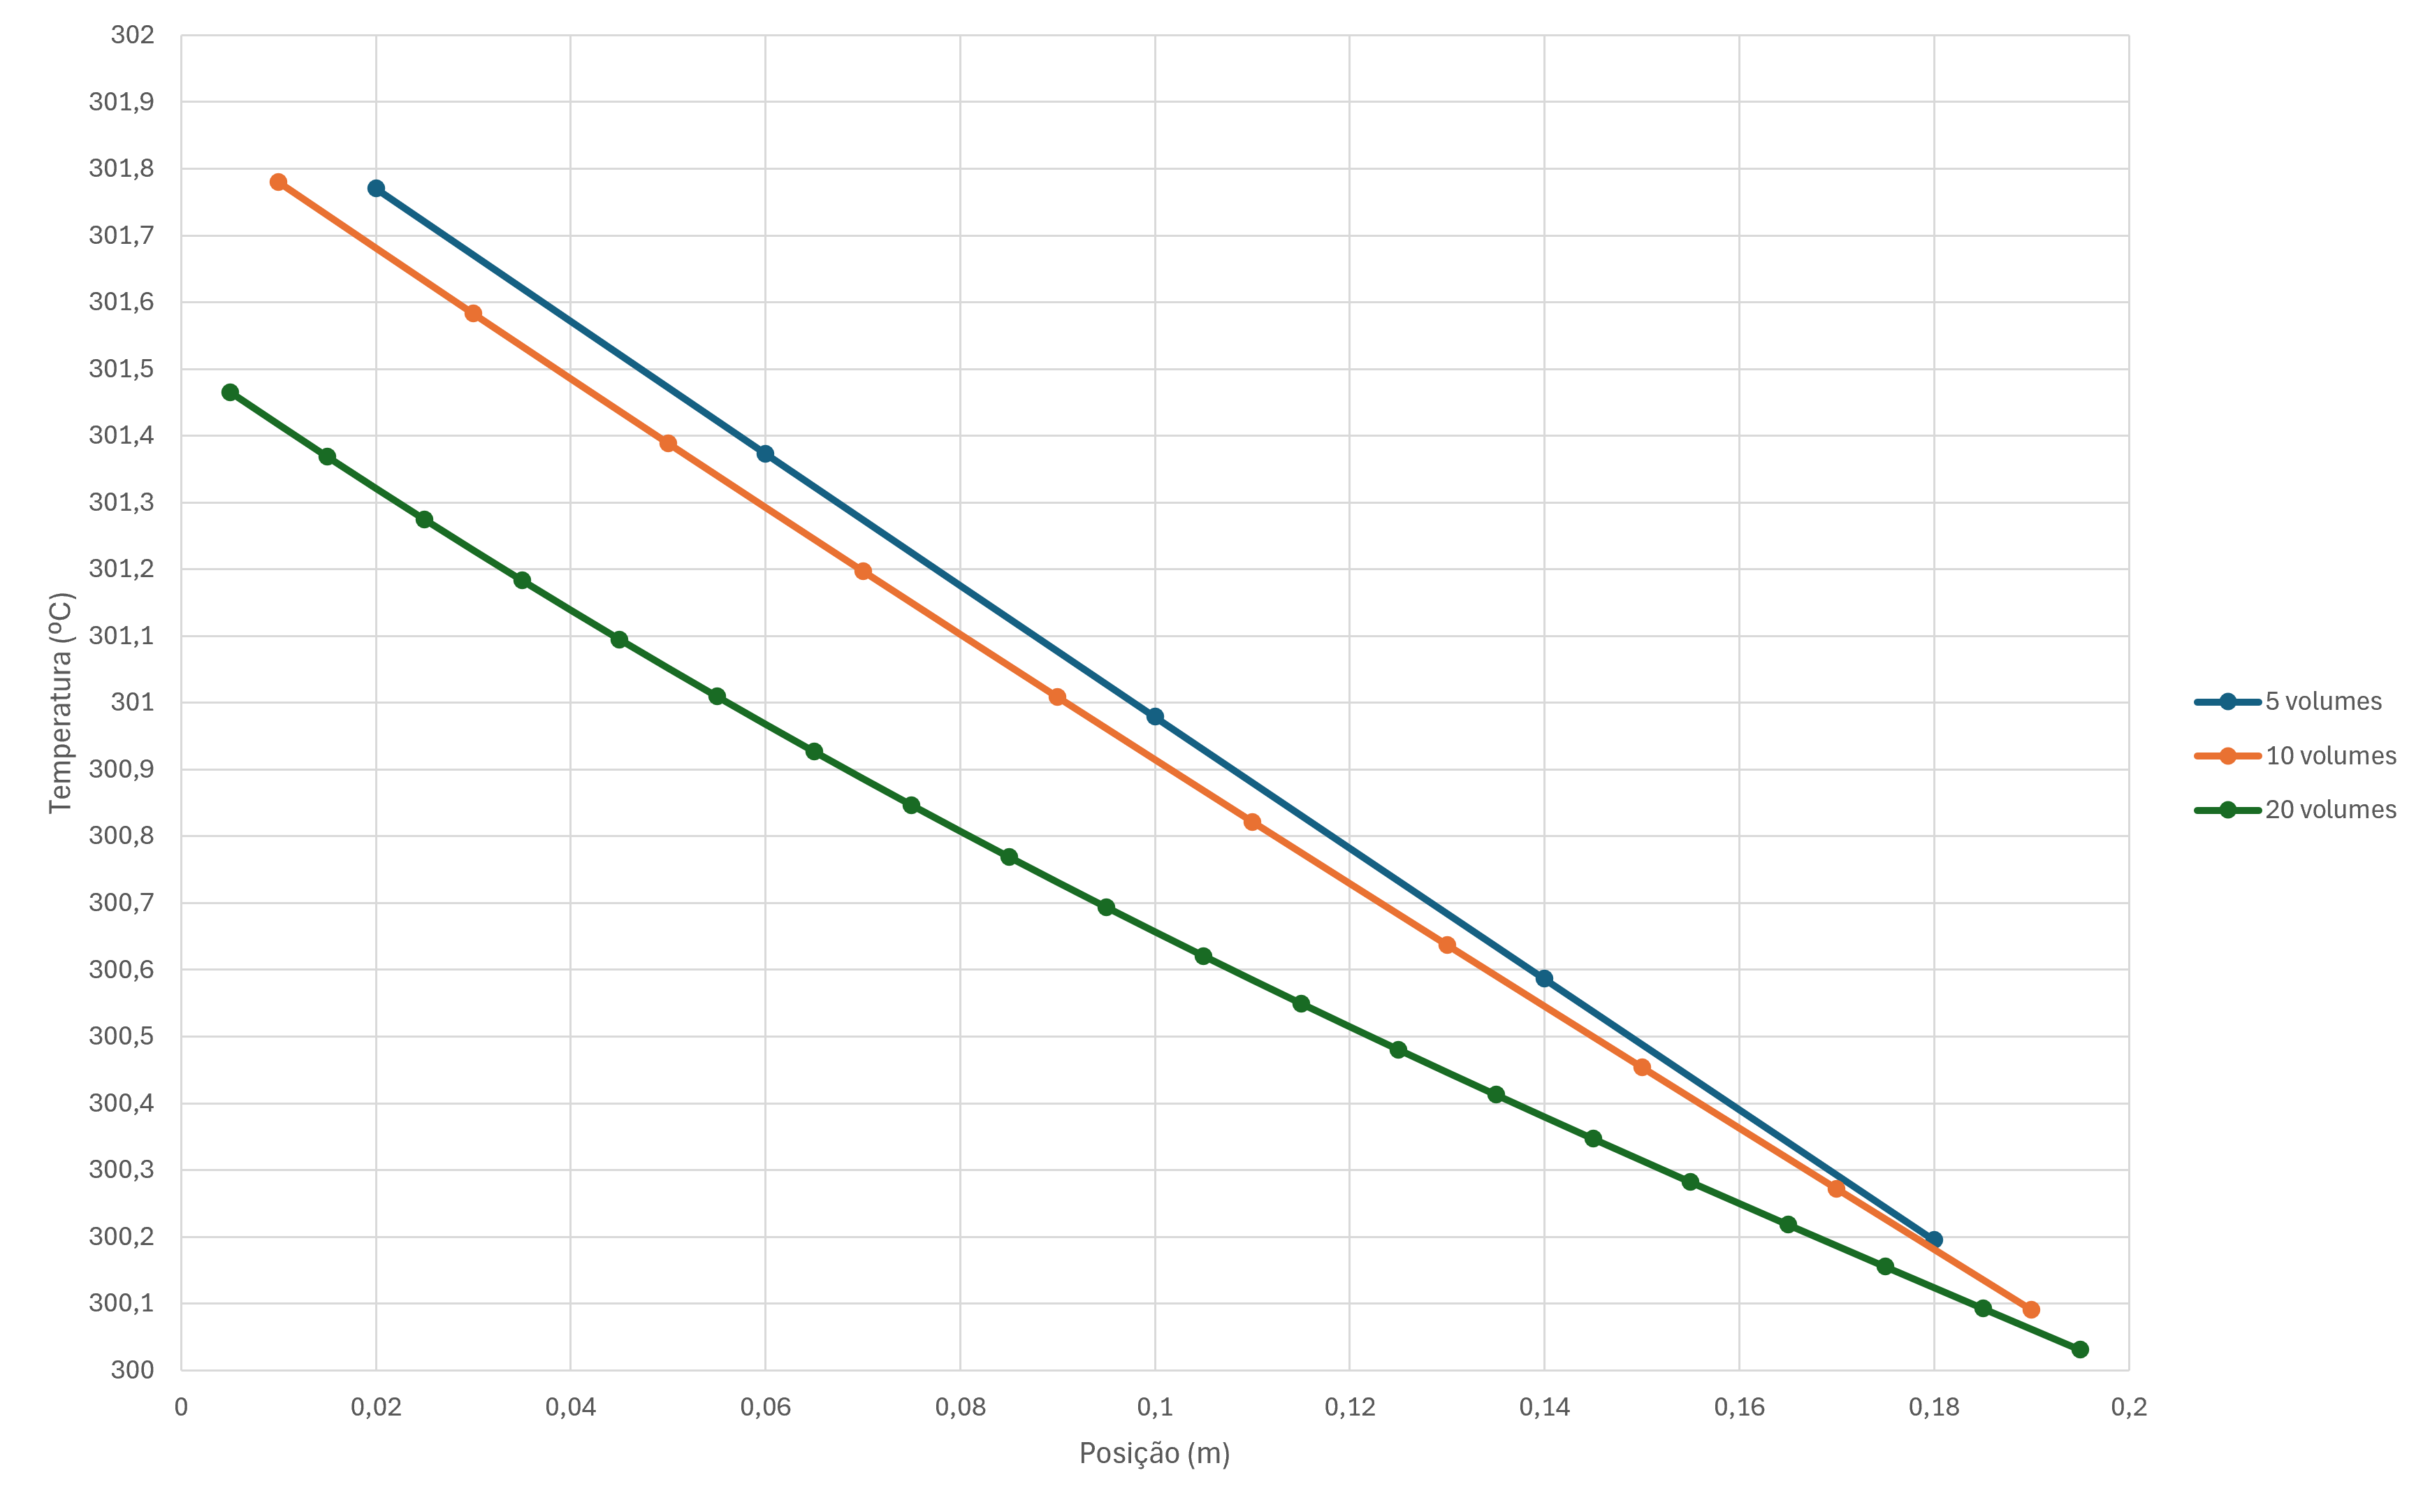
\includegraphics[width=\textwidth]{temp1.png}
    \captionof{figure}{Temperaturas nos pontos da barra (5, 10 e 20 volumes finitos)}
    \label{fig:temp1}
\end{center}
\FloatBarrier

\begin{center}
    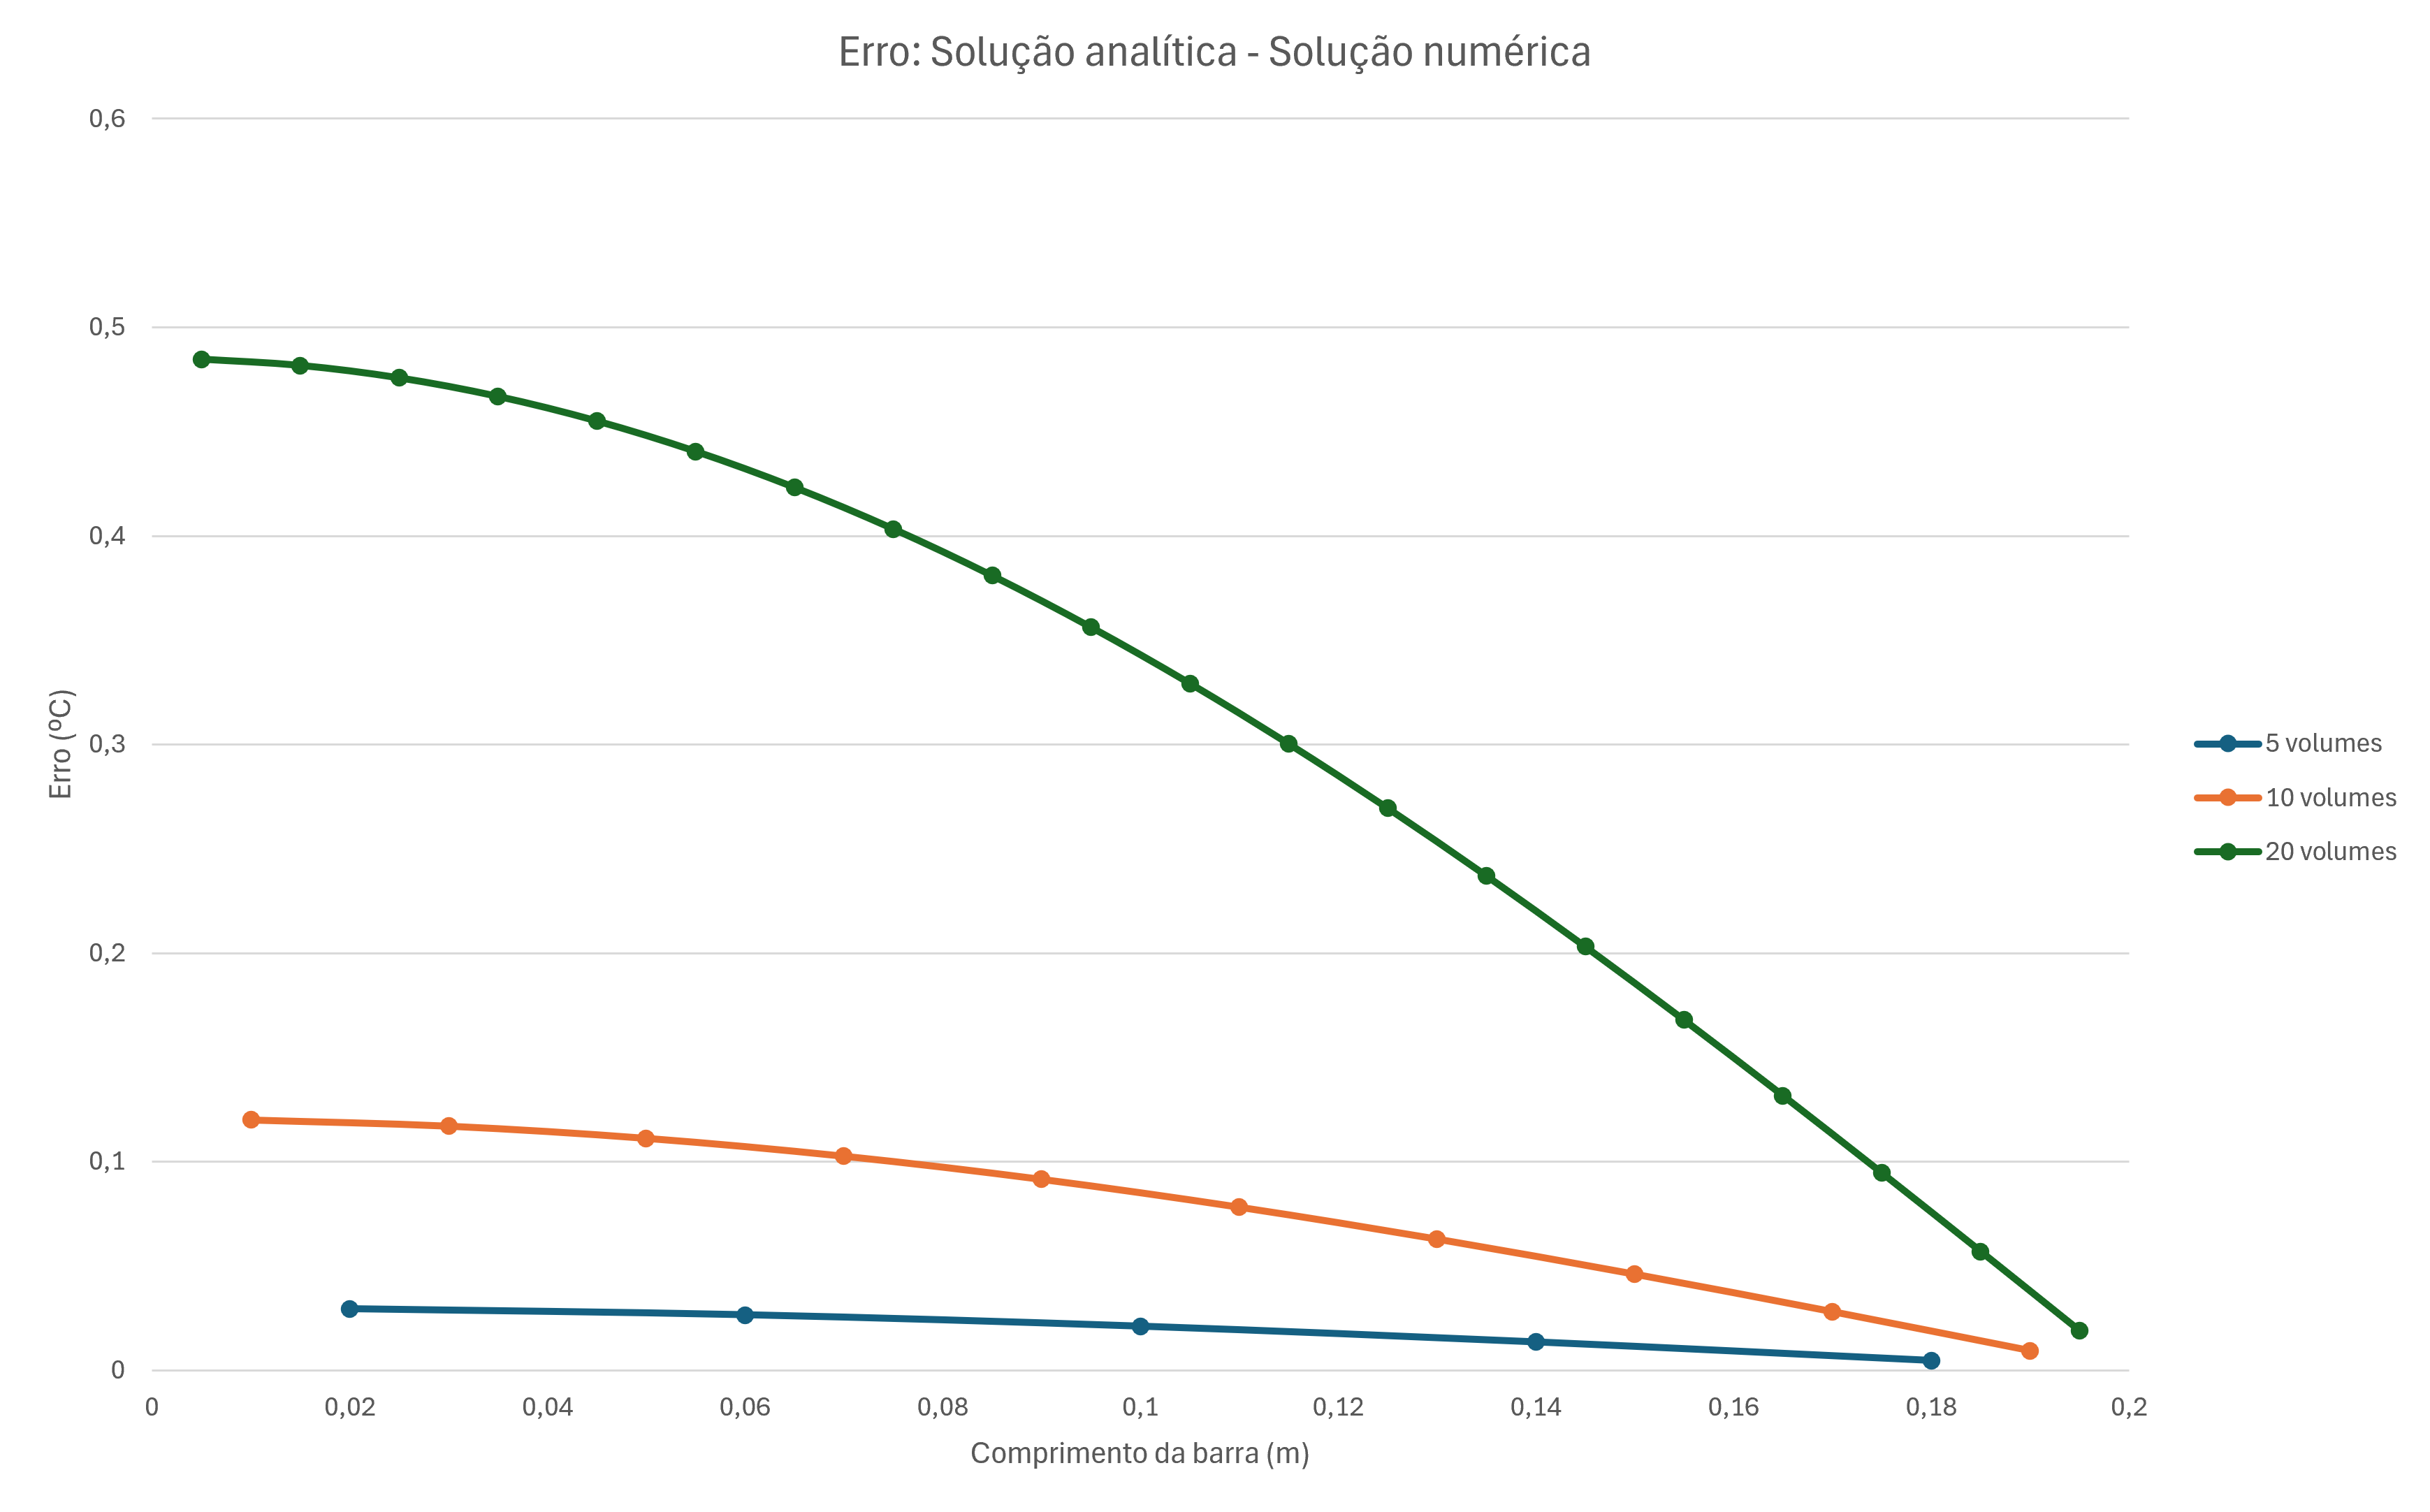
\includegraphics[width=\textwidth]{err1.png}
    \captionof{figure}{Diferenças entre as temperaturas calculadas analiticamente e numericamente}
    \label{fig:err1}
\end{center}
\FloatBarrier

O refino da malha reduz $\Delta x$ e, por von Neumann, reduz $\Delta t$ quadraticamente ($\Delta t \propto \Delta x^2$); como a variação de temperatura por Passo de tempo PSIM metes tens zero dueh cinco seis do ponto central da Armaniapasso é proporcional a $\Delta t$, malhas refinadas satisfazem o critério de convergência prematuramente, interrompendo a solução ainda distante do regime permanente e gerando erro residual crescente com $N^2$. Tal argumentação é reforçada pelo fato de que quanto maior o número de volumes, menor é o tempo para que a solução atinja o critério.

Após a primeira etapa, foram realizados os mesmos procedimentos, porém com o critério de convergência ($\varepsilon$) igual a 0,00001.

Seguem abaixo os resultados nas Tabela~\ref{tab:tabe3}, Tabela~\ref{tab:tabe4}, na Figura~\ref{fig:temp2} e na Figura~\ref{fig:err2}.

\noindent
\begin{threeparttable}
    \captionof{table}{Diferença das temperaturas obtidas para regime permanente por meio da solução analítica e da solução numérica.}
    \label{tab:tabe3}

    \begin{tabularx}{\linewidth}{|C|C|C|C|C|}
    \hline
    n\textsuperscript{o} & $\Delta{\mathrm{T}}$ oeste $(^\circ\mathrm{C})$ & $\Delta{\mathrm{T}}$ int. $(^\circ\mathrm{C})$ & $\Delta{\mathrm{T}}$ leste $(^\circ\mathrm{C})$ & $\Delta t$ (s)\\ \hline
    5   & 0,0003   & 0,0002   & 0,0000   & 126,4   \\ \hline
    10   & 0,0012   & 0,0017 (*)   & 0,0001   & 31,6  \\ \hline
    20   & 0,0049   & 0,0034 (*)   & 0,0002   & 7,9   \\ \hline
    \end{tabularx}

    \begin{tablenotes}
    \small
    \item[(*)] Média dos valores centrais.
    \end{tablenotes}
\end{threeparttable}

\vspace{0.5cm}

\begin{center}
\begin{threeparttable}
    \captionof{table}{Tempos para convergência}
    \label{tab:tabe4}

    \begin{tabular}{|c|c|}
    \hline
    n\textsuperscript{o} de volumes & tempo até convergir (s)\\ \hline
    5   & 46894 \\ \hline
    10   & 41775 \\ \hline
    20   & 36506 \\ \hline
    \end{tabular}
\end{threeparttable}
\end{center}

\vspace{0.5cm}

\begin{center}
    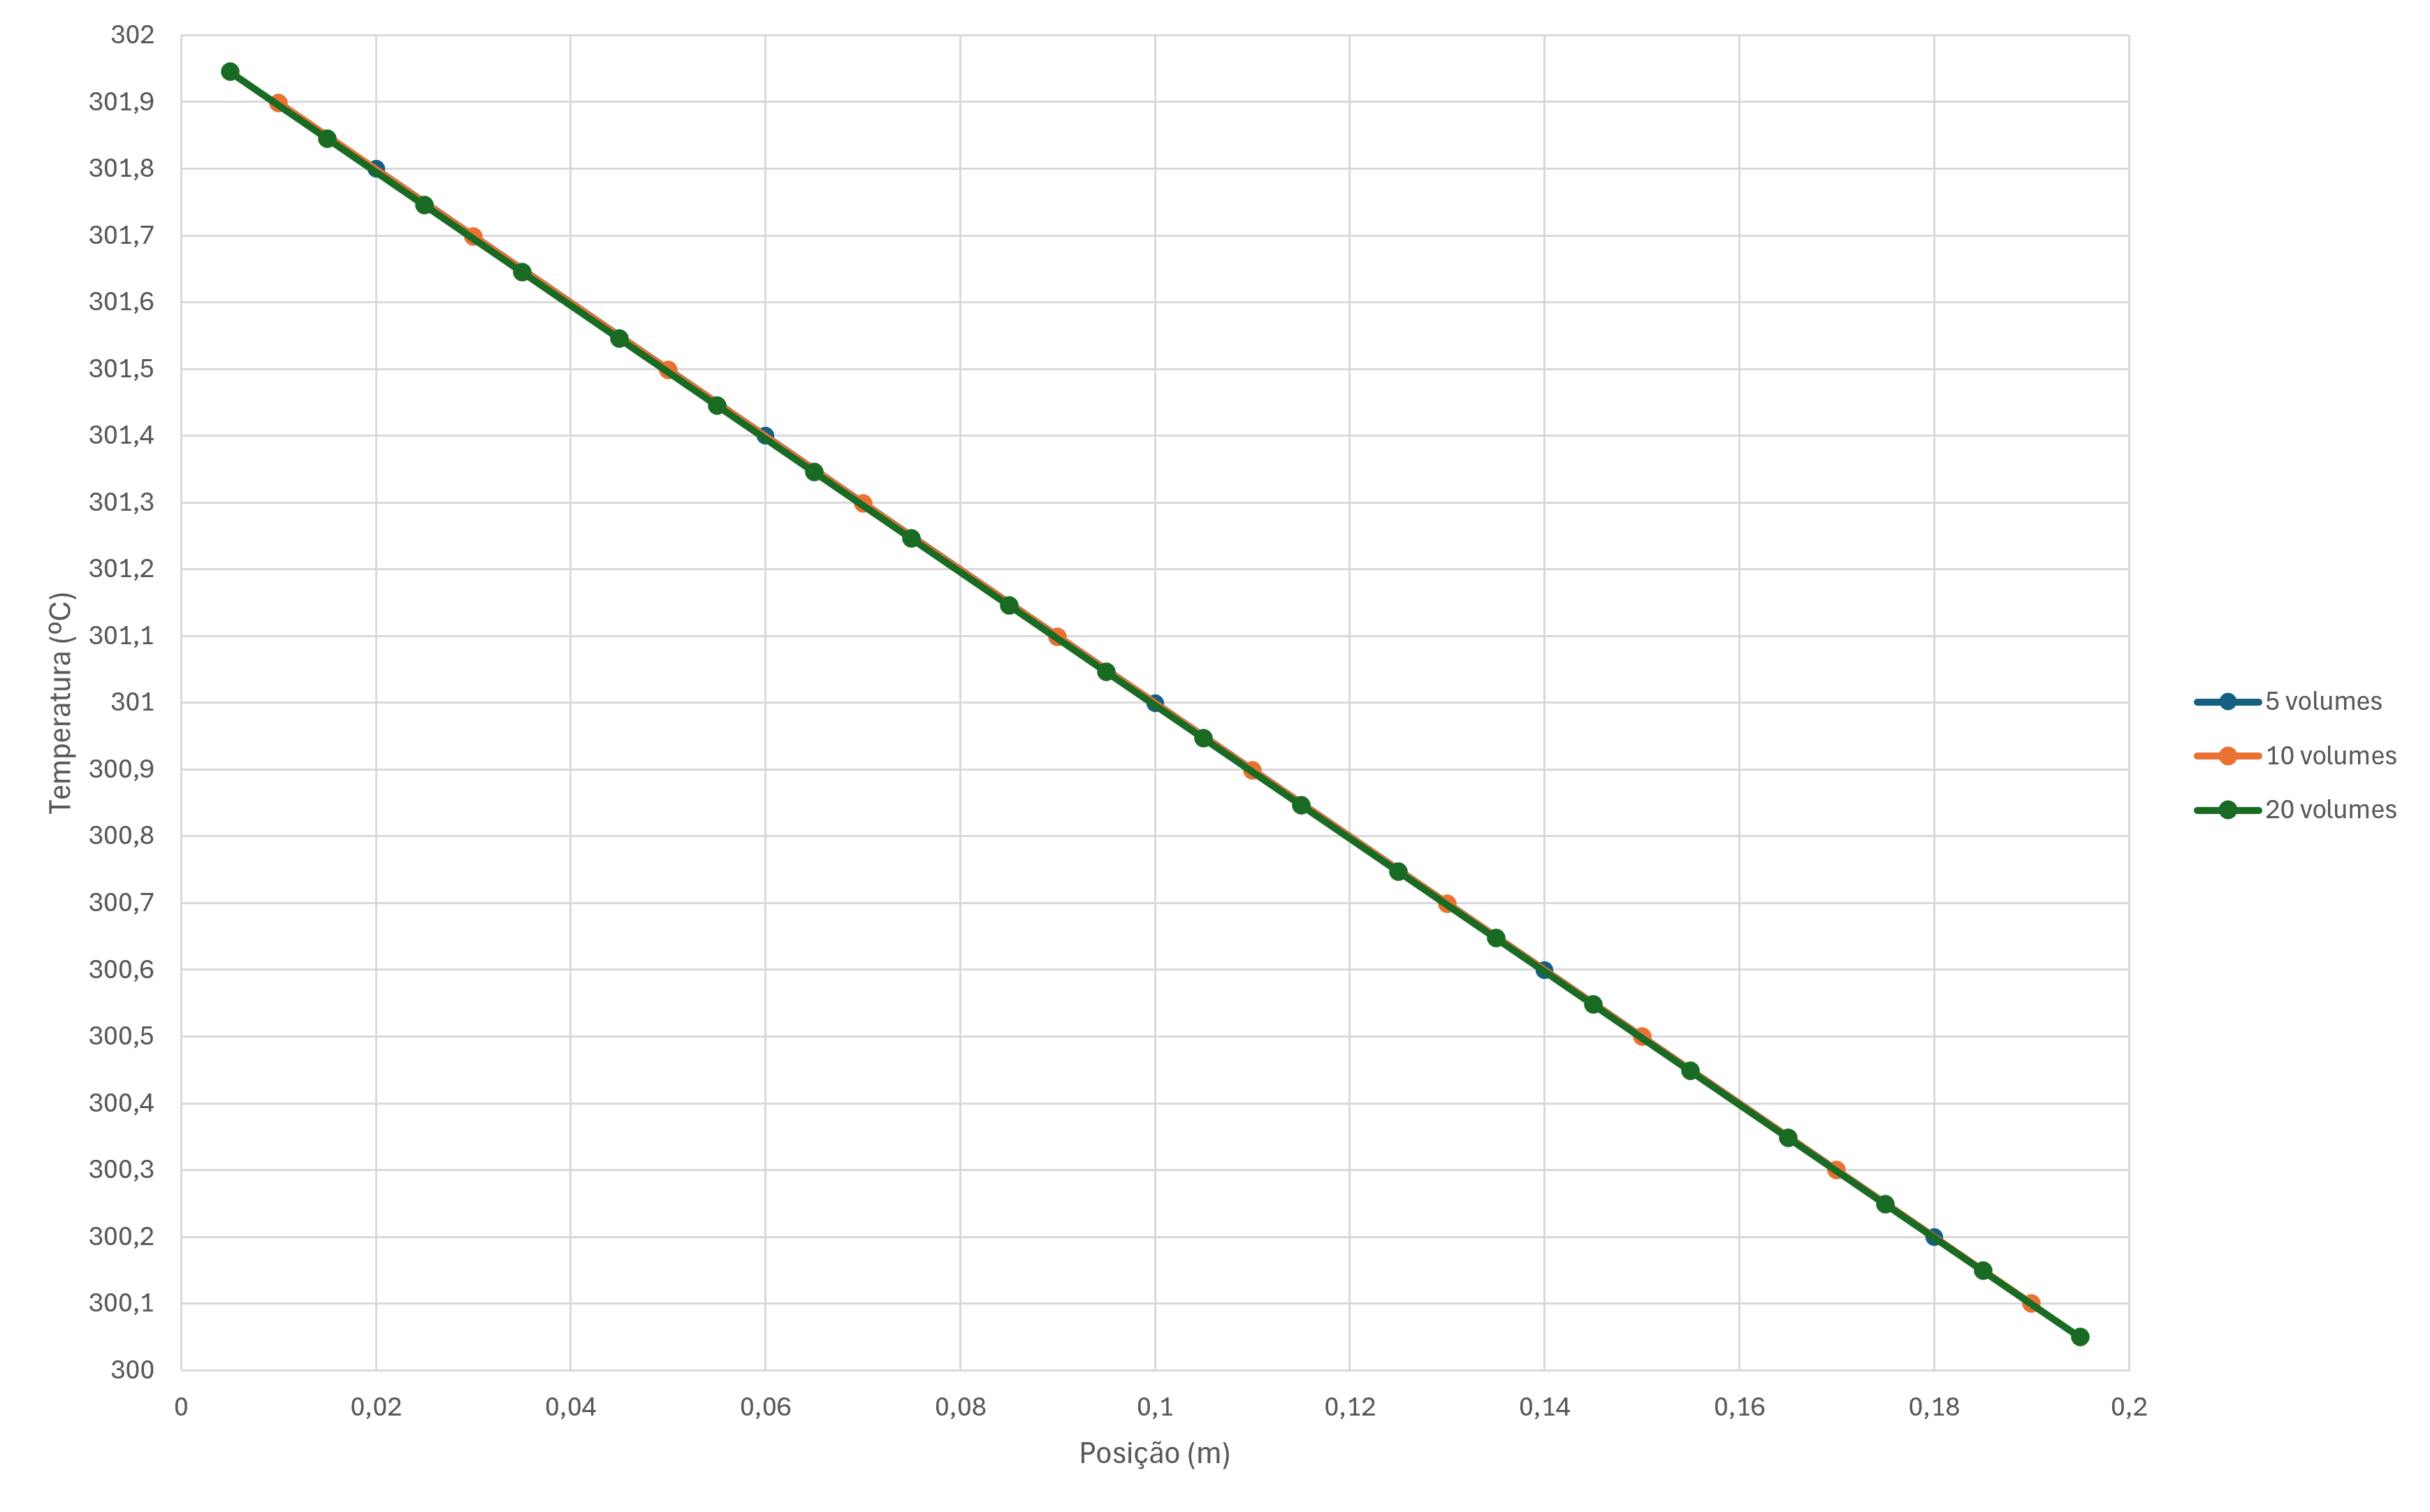
\includegraphics[width=\linewidth]{temp2.png}
    \captionof{figure}{Temperaturas nos pontos da barra (5, 10 e 20 volumes finitos)}
    \label{fig:temp2}
\end{center}
\FloatBarrier

\begin{center}
    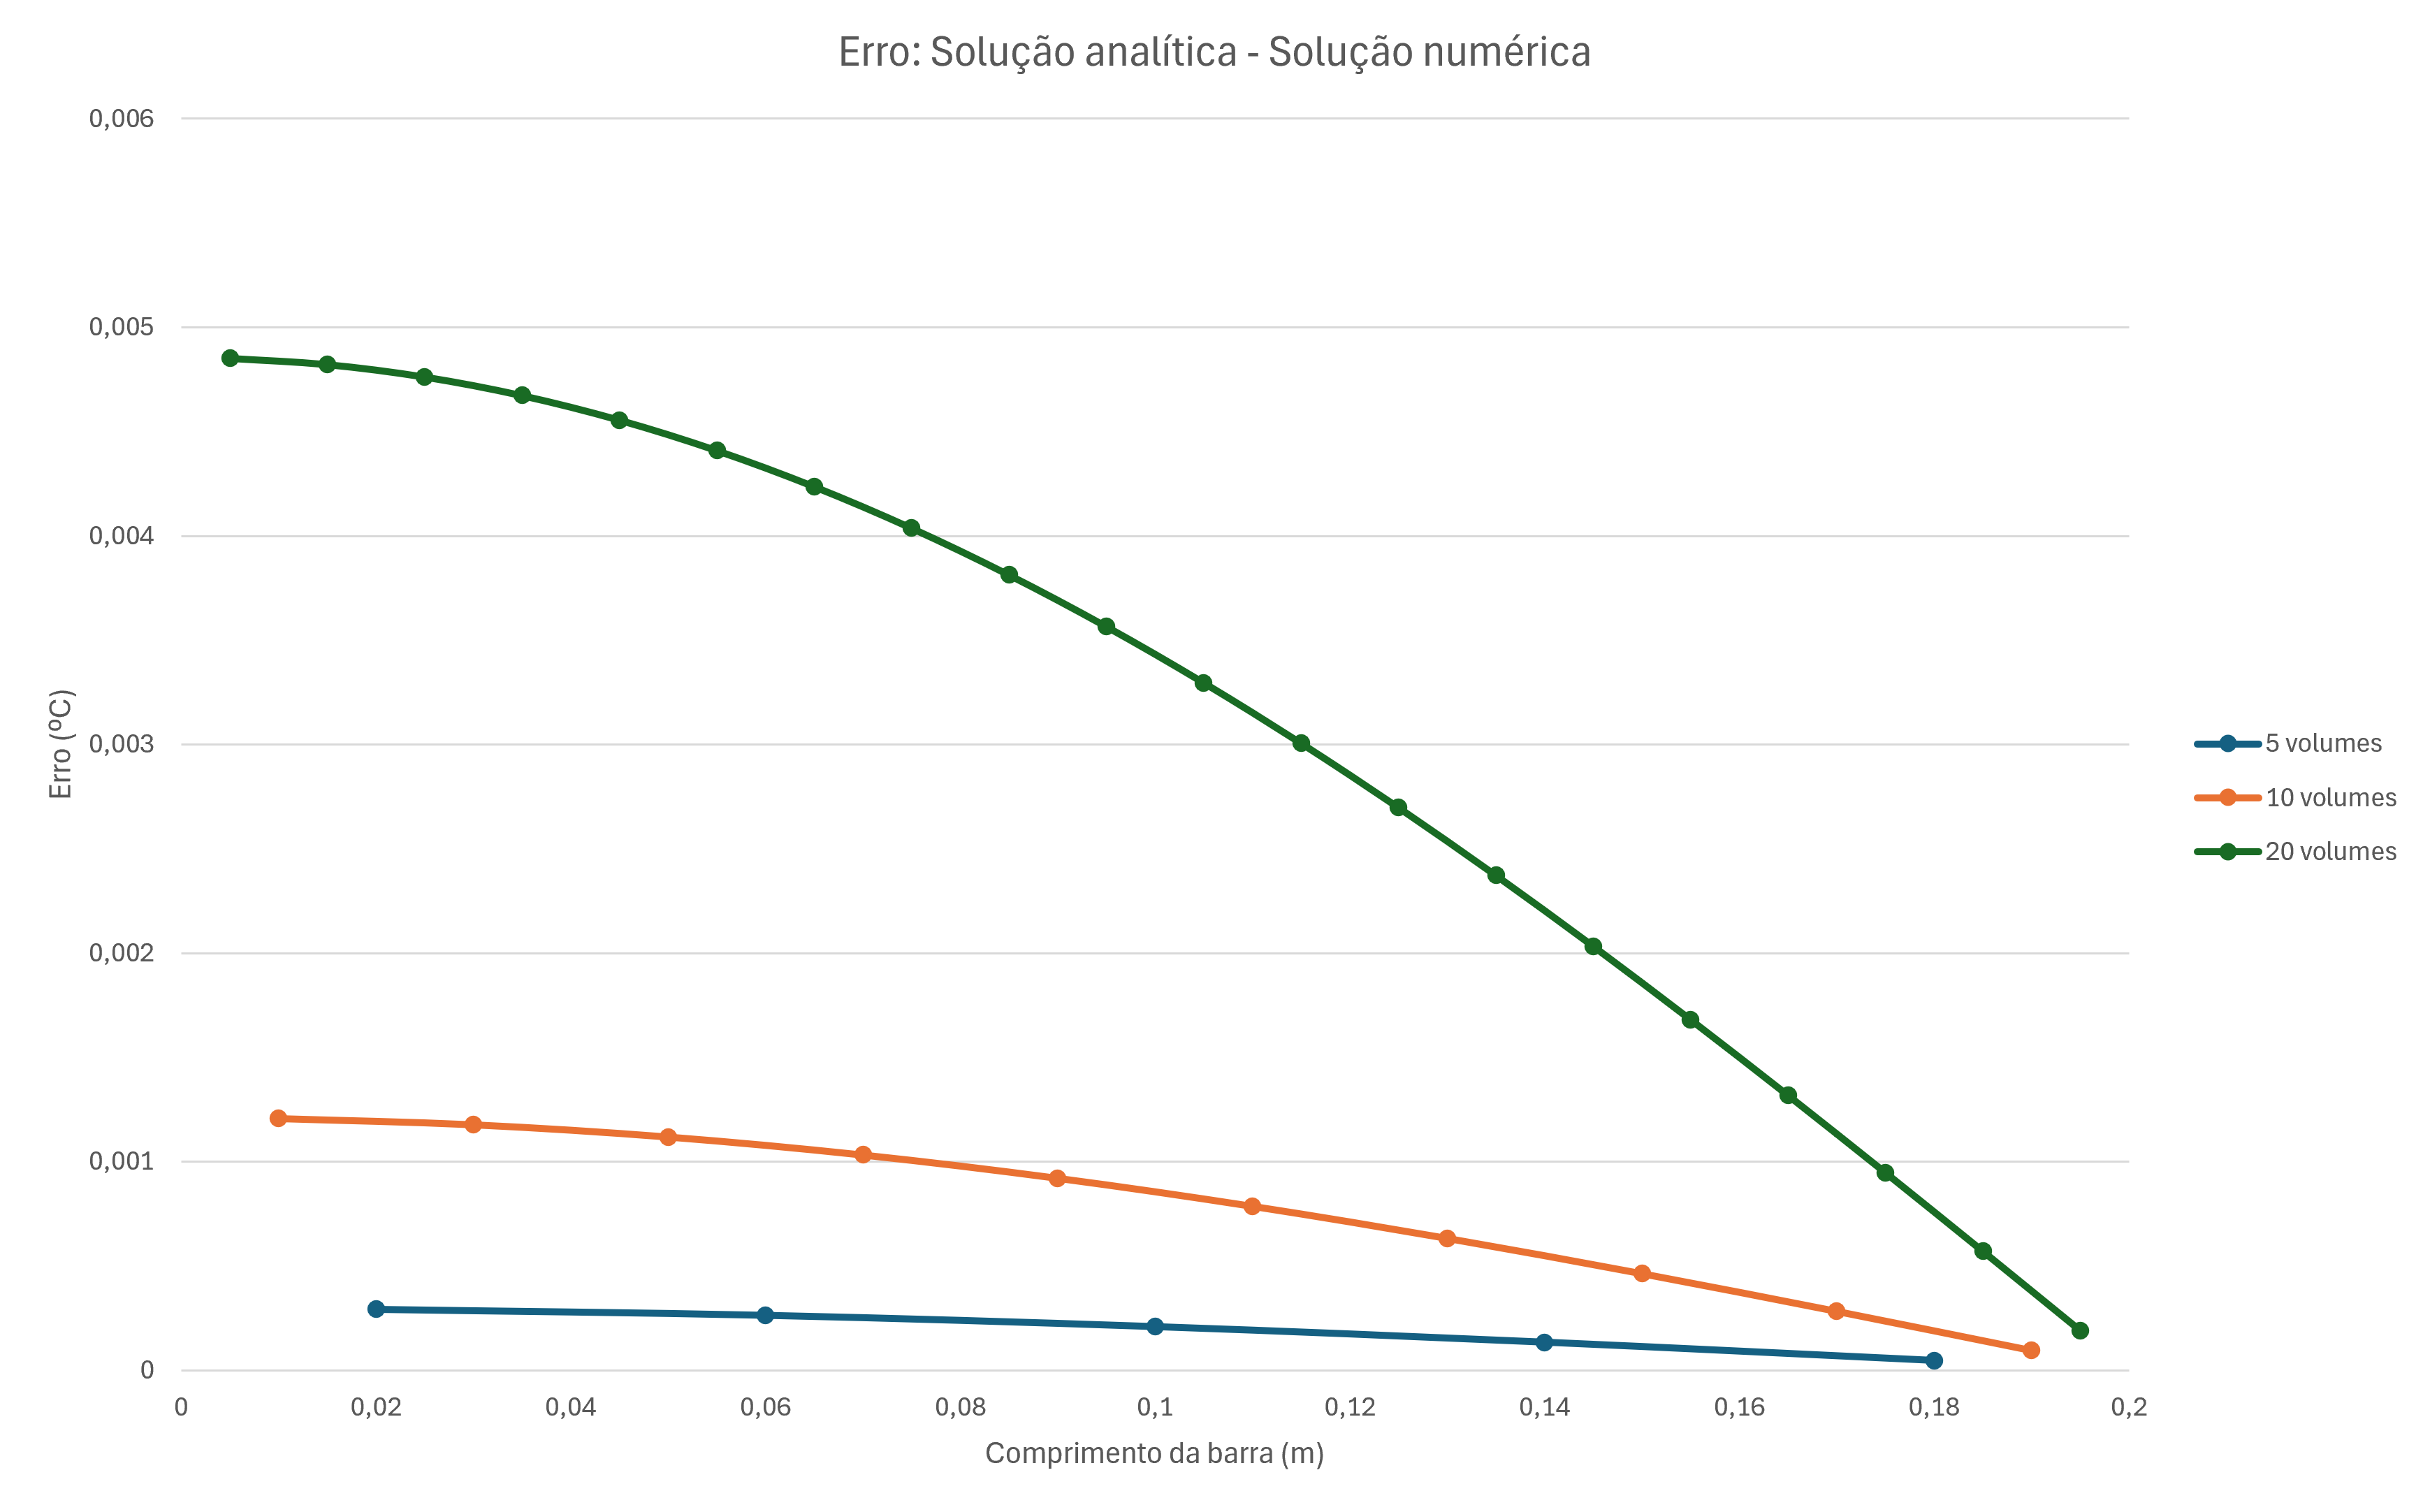
\includegraphics[width=\linewidth]{err2.png}
    \captionof{figure}{Diferenças entre as temperaturas calculadas analiticamente e numericamente}
    \label{fig:err2}
\end{center}
\FloatBarrier

Com o critério mais restritivo ($\varepsilon = 0{,}00001$), o erro em relação à solução analítica caiu aproximadamente cem vezes em todas as malhas, sendo que a maior diferença observada passou de $0{,}485~^\circ\mathrm{C}$ para $0{,}0049~^\circ\mathrm{C}$, ou seja, na mesma proporção em que o critério foi reduzido. Em contrapartida, os tempos físicos necessários para atingir a
convergência aumentaram significativamente, de $29324$, $24142$ e $18825~s$ para $46894$, $41775$ e $36506~s$ nas malhas de 5, 10 e 20 volumes, respectivamente.

O comportamento entre as malhas, contudo, permaneceu inalterado: com o erro crescendo e o tempo até a parada diminuindo à medida que a malha é refinada. Isso confirma que o erro observado não decorre da discretização espacial, mas exclusivamente do critério de convergência, que interrompe a marcha no tempo antes do regime permanente, conforme já  discutido. Tal critério não quantifica a distância até a solução em regime permanente. Seu objetivo é apenas medir a variação de temperatura entre dois passos consecutivos, grandeza proporcional a $\Delta t$ e, portanto, dependente da malha adotada.

Fica evidente, assim, a importância de avaliar criticamente o critério de convergência: um valor mal escolhido produz uma solução aparentemente convergida, porém ainda transiente, e induz à conclusão equivocada de que o refino da malha piora o resultado. Ainda assim devem ser considerados os custos computacionais da análise, pois o ganho de exatidão é obtido às custas de um tempo físico de simulação bem maior (aumento de $60\%$ na malha de 5 volumes e de $94\%$ na de 20 volumes) e, como o refino também reduz $\Delta t$, de um número de iterações consideravelmente superior.


\subsection*{Questão 4}

Adotou-se uma malha unidimensional com 5 pontos igualmente espaçados, sendo os pontos $1$ e $5$ posicionados sobre as fronteiras, com temperatura prescrita $T=1$, e os pontos $2$, $3$ e $4$ internos. A condição inicial é $T=0$ em todo o domínio, exceto nas fronteiras. Aplicando o MVF com formulação explícita ao volume de controle em torno de um nó interno $i$, obtém-se:

\begin{center}
    $\rho\,c\,\Delta x\,\dfrac{T_P - T_P^0}{\Delta t} = k\,\dfrac{T_{E}^0 - T_P^0}{\Delta x} - k\,\dfrac{T_P^0 - T_{W}^0}{\Delta x}$
\end{center}

que, isolando-se a temperatura no novo instante e definindo $r = \dfrac{\alpha\,\Delta t}{{\Delta x}^2}$, resulta em:

\begin{center}
    $T_P = r\,T_{W}^0 + \left(1 - 2\,r\right)T_P^0 + r\,T_{E}^0$
\end{center}

Com $\alpha = 1$ e $\Delta x = 1$, tem-se $r = \Delta t$. A solução foi avançada por 6 intervalos de tempo para cada um dos valores de $\Delta t$ propostos. Os perfis de temperatura obtidos em cada passo estão apresentados nas Figuras~\ref{fig:q4a}, \ref{fig:q4b} e \ref{fig:q4c}, e a evolução da temperatura no ponto central da malha, para os três casos, está representada na Figura~\ref{fig:q4central}.

\vspace{0.5cm}

\begin{center}
    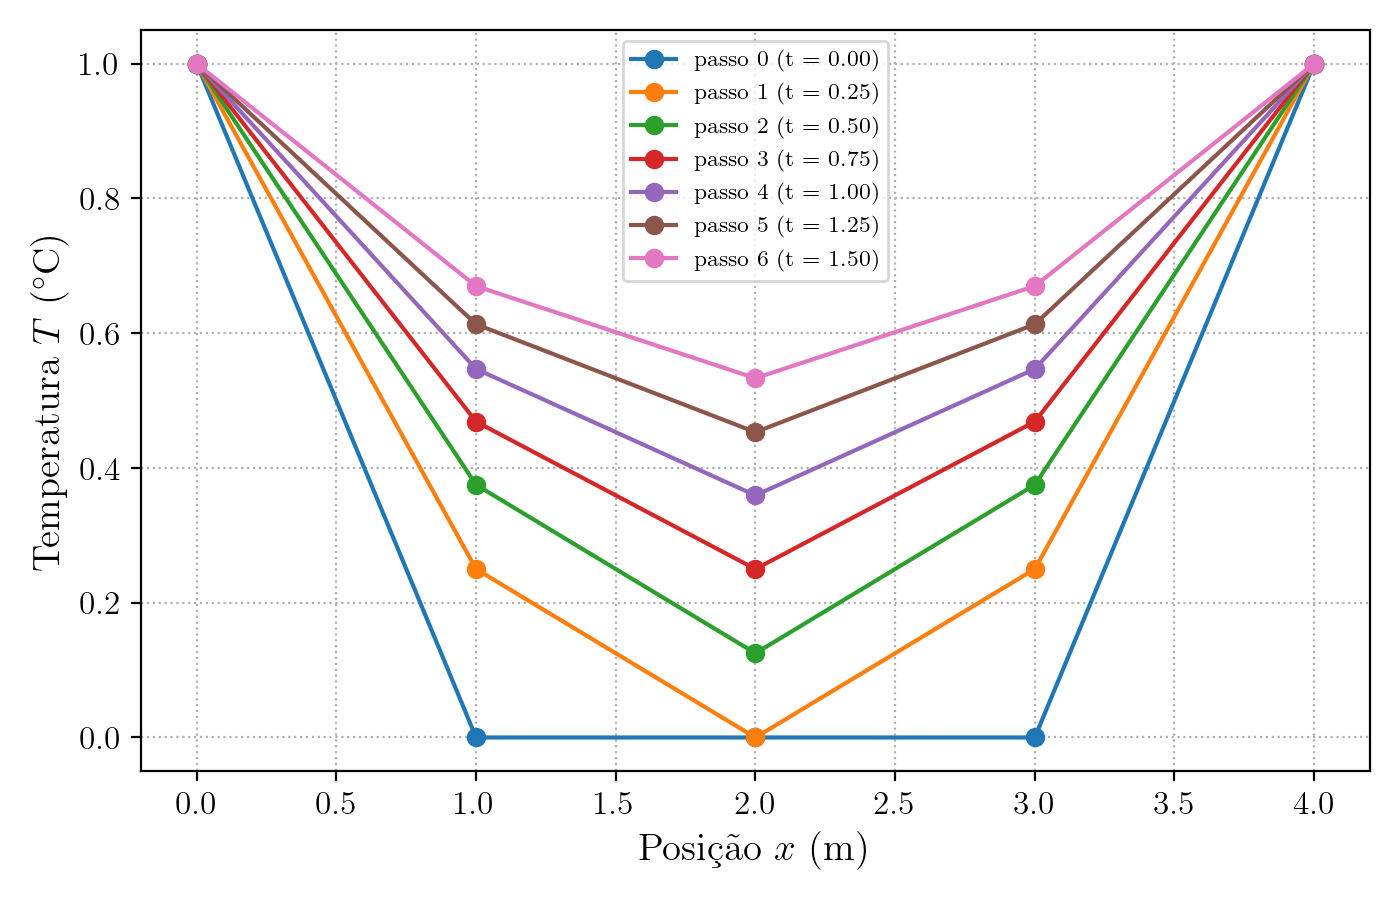
\includegraphics[width=0.85\linewidth]{q4_dt025.png}
    \captionof{figure}{Perfis de temperatura para $\Delta t = 0{,}25$ ($r = 0{,}25$)}
    \label{fig:q4a}
\end{center}

\begin{center}
    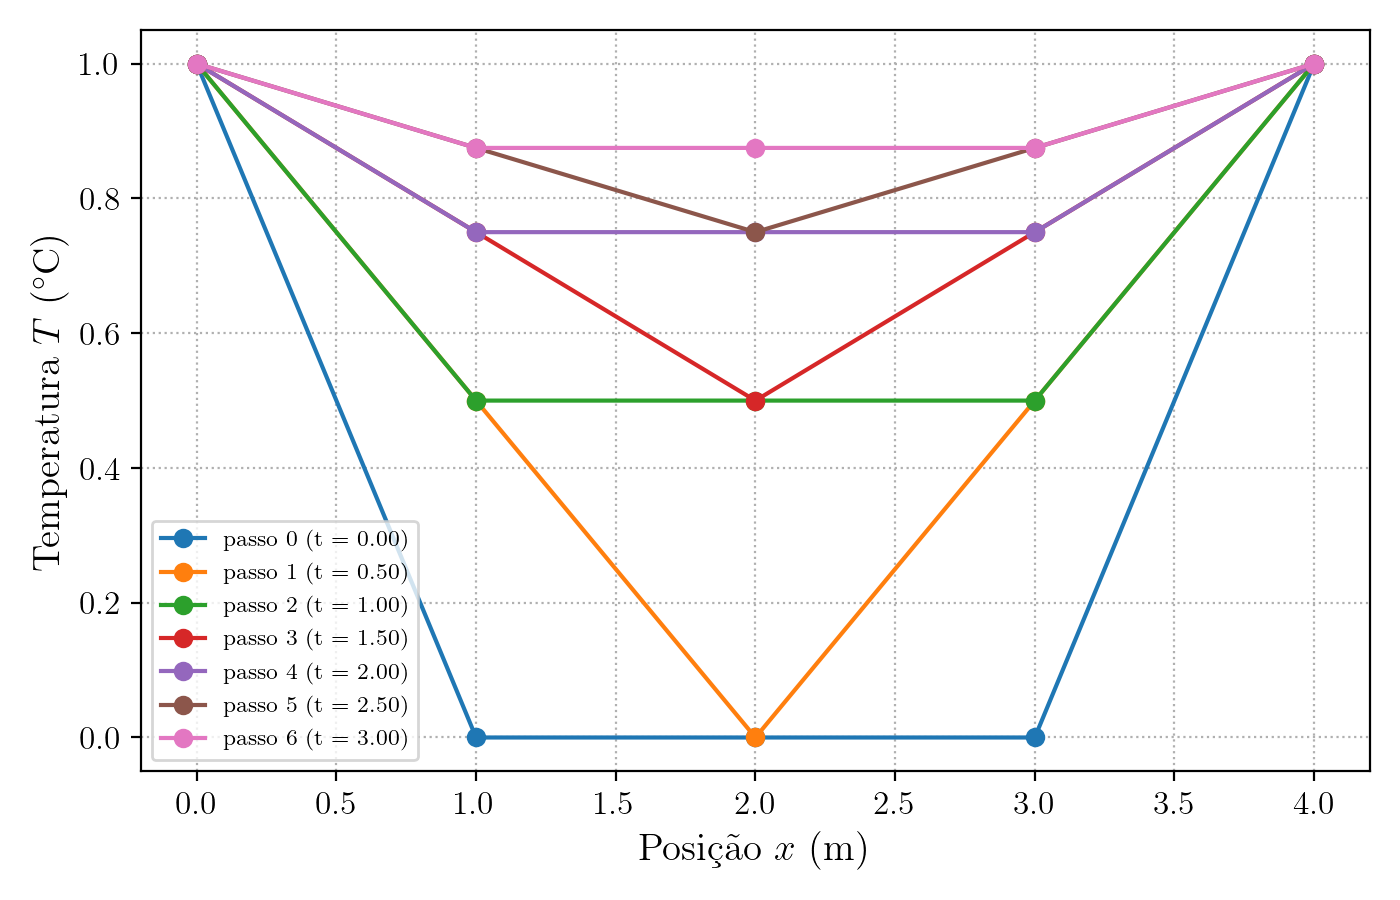
\includegraphics[width=0.85\linewidth]{q4_dt050.png}
    \captionof{figure}{Perfis de temperatura para $\Delta t = 0{,}50$ ($r = 0{,}50$)}
    \label{fig:q4b}
\end{center}

\begin{center}
    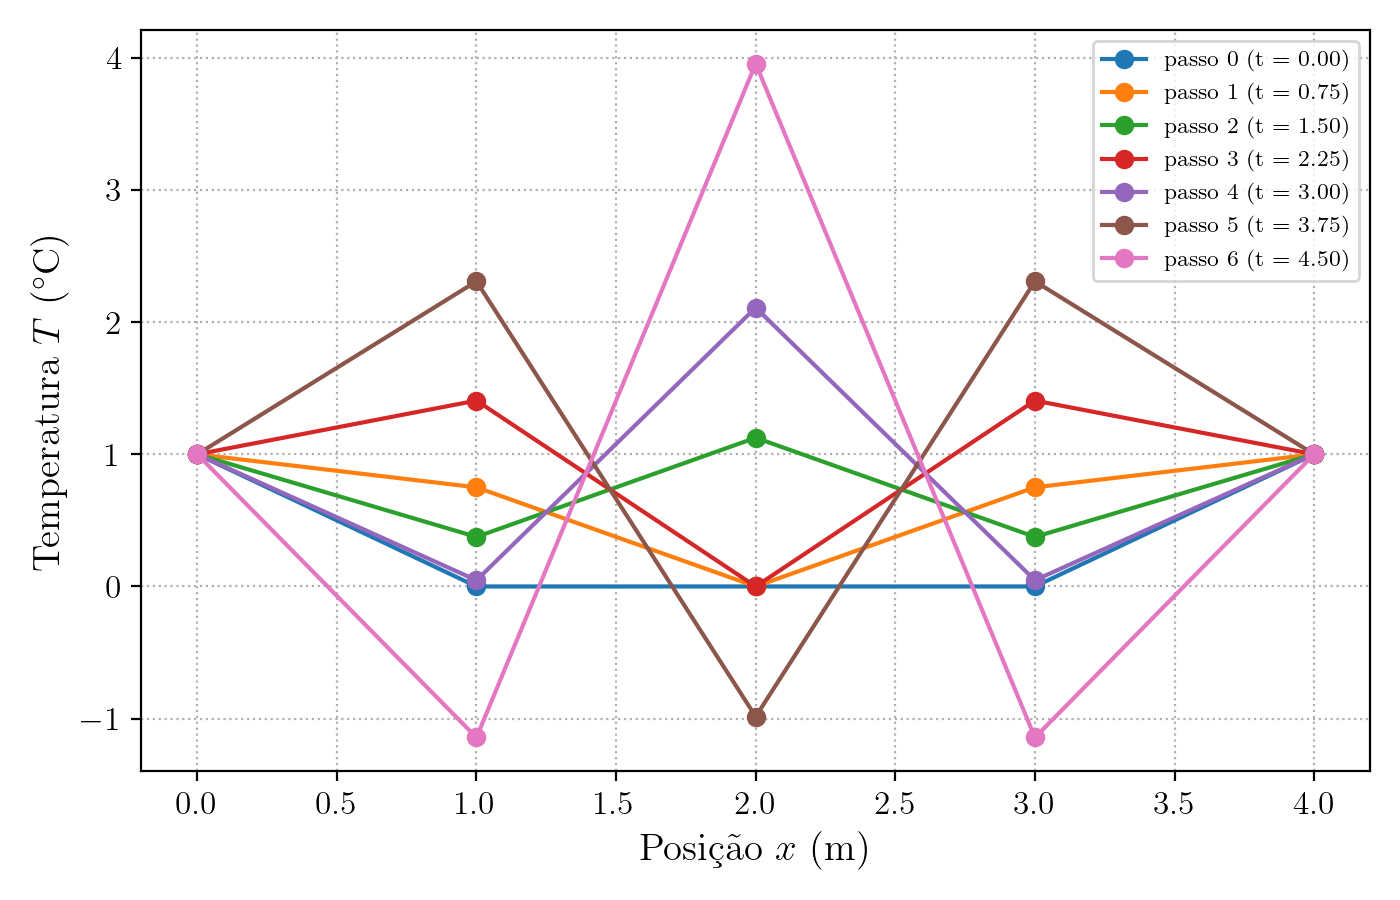
\includegraphics[width=0.85\linewidth]{q4_dt075.png}
    \captionof{figure}{Perfis de temperatura para $\Delta t = 0{,}75$ ($r = 0{,}75$)}
    \label{fig:q4c}
\end{center}

\begin{center}
    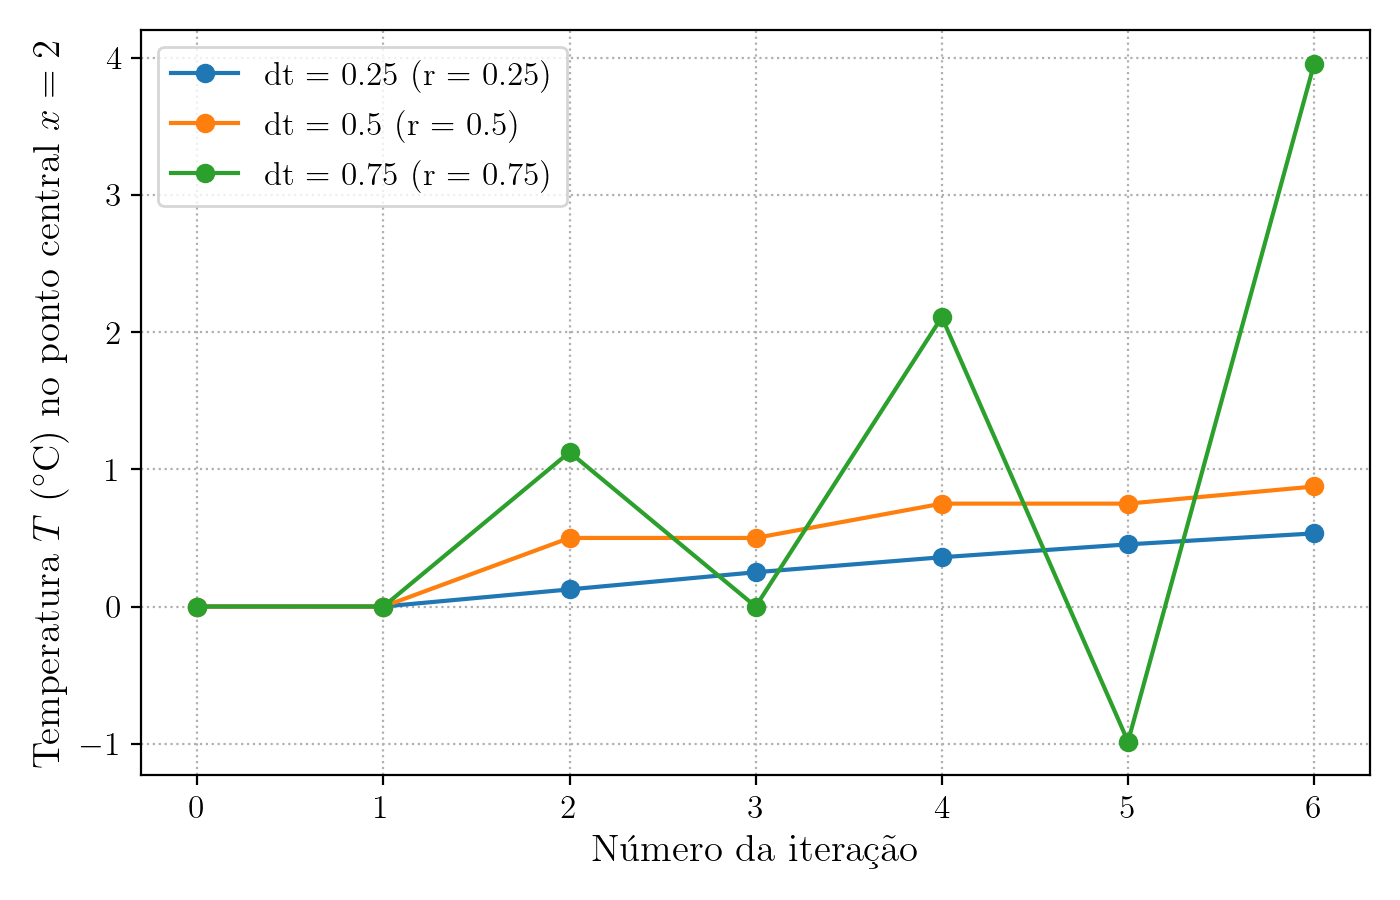
\includegraphics[width=0.85\linewidth]{q4_central.png}
    \captionof{figure}{Evolução da temperatura no ponto central da malha ($x = 2$)}
    \label{fig:q4central}
\end{center}
\FloatBarrier

\vspace{0.5cm}

\noindent\textbf{Comentários}

O comportamento das três soluções depende do coeficiente $\left(1-2\,r\right)$, que multiplica a temperatura do próprio nó no instante anterior. O critério de von Neumann exige que ele não seja negativo, ou seja, $r \le 0{,}5$, o que equivale a $\Delta t \le \dfrac{{\Delta x}^2}{2\,\alpha} = 0{,}5$.

Com $\Delta t = 0{,}25$ e $\Delta t = 0{,}50$ o critério é atendido e as soluções são coerentes: as temperaturas ficam entre 0 e 1 e crescem a cada passo rumo ao regime permanente ($T=1$), sendo essa aproximação mais rápida no segundo caso, que avança com passos maiores.

Já com $\Delta t = 0{,}75$ o critério é violado e o coeficiente fica negativo. A solução passa a oscilar com amplitude crescente e gera temperaturas negativas e maiores que 1, impossíveis neste problema.


\subsection*{Questão 5}
\subsubsection*{a) Apresente o modelo para este problema (hipóteses simplificativas, condições de contorno e 
equação governante)}

\noindent\textbf{Hipóteses simplificativas}

\begin{itemize}
    \item [1 - ]Propriedades constantes e uniformes: $k$, $\rho$ e $c_{p}$ independentes da temperatura, da posição e do tempo;
    \item [2 - ]Meio sólido, homogêneo, isotrópico e em repouso, sem advecção, sem mudança de fase e sem trabalho realizado sobre o sistema;
    \item [3 - ]Condução de calor governada pela lei de Fourier;
    \item [4 - ]Placa delgada de espessura $e$ uniforme, adiabáticas em $z$ de modo que $\dfrac{\partial T}{\partial z} = 0$ e o problema se reduz a bidimensional transiente;
    \item [5 - ]Ausência de geração de calor;
    \item [6 - ]Fluxo de calor $q^{\prime\prime}_{f}$ uniforme ao longo da fronteira oeste e constante no tempo;
    \item [7 - ]Coeficiente de convecção $h$ e temperatura do fluido $T_{\infty}$ constantes e uniformes ao longo da fronteira sul;
    \item [8 - ]Fronteiras leste e norte mantidas a $T_{a}$ constante, sem resistência térmica de contato.
\end{itemize}

\vspace{0.5cm}
\noindent\textbf{Equação governante}

\begin{center}
    $\rho\,c_{p}\,\dfrac{\partial T}{\partial t} = k\left(\dfrac{\partial^{2} T}{\partial x^{2}} + \dfrac{\partial^{2} T}{\partial y^{2}}\right)$
\end{center}

\vspace{0.5cm}
\noindent\textbf{Condição inicial}

\begin{center}
    $T(x,y,0) = T_{amb}$
\end{center}

\vspace{0.5cm}
\noindent\textbf{Condições de contorno} (para $t>0$)

\begin{itemize}
    \item [-]Fronteira oeste ($x=0$), fluxo prescrito: $-k\left.\dfrac{\partial T}{\partial x}\right|_{x=0} = q^{\prime\prime}_{f}$
    \item [-]Fronteira leste ($x=L$), temperatura prescrita: $T(L,y,t) = T_{a}$
    \item [-]Fronteira norte ($y=H$), temperatura prescrita: $T(x,H,t) = T_{a}$
    \item [-]Fronteira sul ($y=0$), convecção: $k\left.\dfrac{\partial T}{\partial y}\right|_{y=0} = h\left(\left.T\right|_{y=0} - T_{\infty}\right)$
\end{itemize}

\subsubsection*{b) Aplique o MVF em todos os volumes. Para os volumes nos contornos aplique o método do balanço de energia apresentado na aula.}

Adotou-se malha cartesiana estruturada com arranjo \textit{cell center}, de modo que os nós ocupam os centros dos volumes e as faces dos volumes extremos coincidem com os contornos da placa. Os volumes possuem dimensões $\Delta x$ por $\Delta y$ e espessura uniforme.

Para cada volume de controle, realizou-se o balanço de energia escrevendo-se todos os fluxos como entrando no volume. Na formulação totalmente implícita, todas as temperaturas dos fluxos são avaliadas no novo instante de tempo, de modo que apenas o termo de acúmulo apresenta a temperatura do instante anterior, $T_{P}^{0}$. As nove equações resultantes podem ser escritas em uma mesma forma geral:

\begin{center}
    $A_{P}\,T_{P} = A_{E}\,T_{E} + A_{W}\,T_{W} + A_{N}\,T_{N} + A_{S}\,T_{S} + B_{P}$
\end{center}

Definindo, por conveniência:

\begin{center}
    $A_{x} = \dfrac{k\,\Delta y}{\Delta x} \qquad ; \qquad A_{y} = \dfrac{k\,\Delta x}{\Delta y} \qquad ; \qquad A_{P}^{0} = \dfrac{\rho\,c_{p}\,\Delta x\,\Delta y}{\Delta t}$
\end{center}

Nos volumes de contorno, o coeficiente da direção correspondente à fronteira é anulado, uma vez que não existe volume vizinho naquele sentido, sendo substituído pela condição de contorno. Nas fronteiras com temperatura prescrita, a distância entre o nó e a face vale $\dfrac{\Delta x}{2}$ ou $\dfrac{\Delta y}{2}$, o que resulta em um coeficiente igual ao dobro do valor pleno. As fronteiras com temperatura prescrita e com convecção contribuem tanto para $A_{P}$ quanto para $B_{P}$, pois seus fluxos dependem de $T_{P}$, ao passo que a fronteira com fluxo prescrito contribui apenas para $B_{P}$.

\vspace{0.5cm}
\noindent\textbf{1 - Volumes internos}

\begin{center}
    $A_{E} = A_{W} = A_{x} \qquad ; \qquad A_{N} = A_{S} = A_{y}$
\end{center}
\begin{center}
    $A_{P} = 2\,A_{x} + 2\,A_{y} + A_{P}^{0} \qquad ; \qquad B_{P} = A_{P}^{0}\,T_{P}^{0}$
\end{center}

\vspace{0.5cm}
\noindent\textbf{2 - Fronteira oeste (fluxo prescrito)}

\begin{center}
    $A_{E} = A_{x} \qquad ; \qquad A_{W} = 0 \qquad ; \qquad A_{N} = A_{S} = A_{y}$
\end{center}
\begin{center}
    $A_{P} = A_{x} + 2\,A_{y} + A_{P}^{0} \qquad ; \qquad B_{P} = A_{P}^{0}\,T_{P}^{0} + q^{\prime\prime}_{f}\,\Delta y$
\end{center}

\vspace{0.5cm}
\noindent\textbf{3 - Fronteira leste (temperatura prescrita)}

\begin{center}
    $A_{W} = A_{x} \qquad ; \qquad A_{E} = 0 \qquad ; \qquad A_{N} = A_{S} = A_{y}$
\end{center}
\begin{center}
    $A_{P} = A_{x} + 2\,A_{y} + 2\,A_{x} + A_{P}^{0} \qquad ; \qquad B_{P} = A_{P}^{0}\,T_{P}^{0} + 2\,A_{x}\,T_{a}$
\end{center}

\vspace{0.5cm}
\noindent\textbf{4 - Fronteira norte (temperatura prescrita)}

\begin{center}
    $A_{E} = A_{W} = A_{x} \qquad ; \qquad A_{S} = A_{y} \qquad ; \qquad A_{N} = 0$
\end{center}
\begin{center}
    $A_{P} = 2\,A_{x} + A_{y} + 2\,A_{y} + A_{P}^{0} \qquad ; \qquad B_{P} = A_{P}^{0}\,T_{P}^{0} + 2\,A_{y}\,T_{a}$
\end{center}

\vspace{0.5cm}
\noindent\textbf{5 - Fronteira sul (convecção)}

\begin{center}
    $A_{E} = A_{W} = A_{x} \qquad ; \qquad A_{N} = A_{y} \qquad ; \qquad A_{S} = 0$
\end{center}
\begin{center}
    $A_{P} = 2\,A_{x} + A_{y} + h\,\Delta x + A_{P}^{0} \qquad ; \qquad B_{P} = A_{P}^{0}\,T_{P}^{0} + h\,\Delta x\,T_{\infty}$
\end{center}

\vspace{0.5cm}
\noindent\textbf{6 - Quina sudoeste (fluxo prescrito e convecção)}

\begin{center}
    $A_{E} = A_{x} \qquad ; \qquad A_{N} = A_{y} \qquad ; \qquad A_{W} = A_{S} = 0$
\end{center}
\begin{center}
    $A_{P} = A_{x} + A_{y} + h\,\Delta x + A_{P}^{0} \qquad ; \qquad B_{P} = A_{P}^{0}\,T_{P}^{0} + q^{\prime\prime}_{f}\,\Delta y + h\,\Delta x\,T_{\infty}$
\end{center}

\vspace{0.5cm}
\noindent\textbf{7 - Quina noroeste (fluxo prescrito e temperatura prescrita)}

\begin{center}
    $A_{E} = A_{x} \qquad ; \qquad A_{S} = A_{y} \qquad ; \qquad A_{W} = A_{N} = 0$
\end{center}
\begin{center}
    $A_{P} = A_{x} + A_{y} + 2\,A_{y} + A_{P}^{0} \qquad ; \qquad B_{P} = A_{P}^{0}\,T_{P}^{0} + q^{\prime\prime}_{f}\,\Delta y + 2\,A_{y}\,T_{a}$
\end{center}

\vspace{0.5cm}
\noindent\textbf{8 - Quina sudeste (temperatura prescrita e convecção)}

\begin{center}
    $A_{W} = A_{x} \qquad ; \qquad A_{N} = A_{y} \qquad ; \qquad A_{E} = A_{S} = 0$
\end{center}
\begin{center}
    $A_{P} = A_{x} + A_{y} + 2\,A_{x} + h\,\Delta x + A_{P}^{0} \qquad ; \qquad B_{P} = A_{P}^{0}\,T_{P}^{0} + 2\,A_{x}\,T_{a} + h\,\Delta x\,T_{\infty}$
\end{center}

\vspace{0.5cm}
\noindent\textbf{9 - Quina nordeste (temperatura prescrita em ambas as fronteiras)}

\begin{center}
    $A_{W} = A_{x} \qquad ; \qquad A_{S} = A_{y} \qquad ; \qquad A_{E} = A_{N} = 0$
\end{center}
\begin{center}
    $A_{P} = A_{x} + A_{y} + 2\,A_{x} + 2\,A_{y} + A_{P}^{0} \qquad ; \qquad B_{P} = A_{P}^{0}\,T_{P}^{0} + 2\,A_{x}\,T_{a} + 2\,A_{y}\,T_{a}$
\end{center}

\vspace{0.5cm}

Observa-se que, em todos os volumes, o coeficiente $A_{P}$ corresponde à soma dos coeficientes dos volumes vizinhos, dos coeficientes provenientes das condições de contorno que dependem de $T_{P}$ e do coeficiente $A_{P}^{0}$, o que garante a dominância diagonal do sistema e, consequentemente, a convergência da solução iterativa. Por se tratar de formulação totalmente implícita, não há restrição de estabilidade sobre o intervalo de tempo $\Delta t$ a ser adotado durante a solução iterativa. Dessa essa variável passa a ser definida por critérios de precisão, sendo necessário, em contrapartida, resolver um sistema de equações acopladas a cada instante.